\newpage
\section{LITERATURE REVIEW}

\subsection{Human Audio Perception}

The human ear is an exceedingly complex organ.  To make matters even more difficult, the information from two ears is combined in a perplexing neural network,
the human brain. \cite{smith2013}

\textit{Figure 1} illustrates the major structures and processes that comprise the human ear. The outer ear is composed of two parts, the visible flap of skin and
cartilage attached to the side of the head, and the ear canal, a tubeabout 0.5 cm in diameter extending about three cm into the head. These structures direct environmental
sounds to the sensitive middle and inner ear organs located safely inside of the skull bones. Stretched across the end of the ear canal is a thin sheet of tissue called the
tympanic membrane or eardrum. Sound waves striking the tympanic membrane cause it to vibrate. The middle ear is a set of small bones that transfer this vibration to the cochlea
(inner ear) where it is converted to neural impulses. The cochlea is a liquid filled tube roughly two mm in diameter and three cm in length.
\begin{figure}[h]
        \centering
        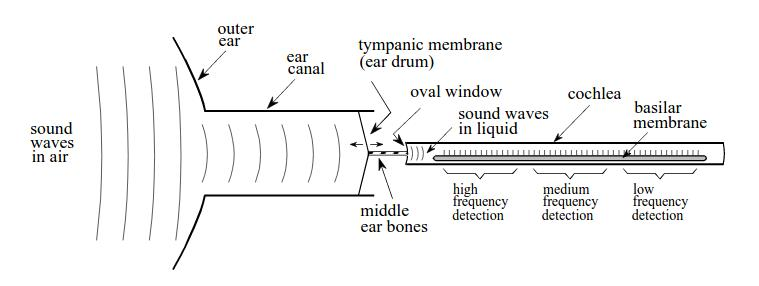
\includegraphics[width=150mm]{resources/humanear.jpg}
        \caption{Functional Diagram of Human Ear}
        \label{fig:figure1}
\end{figure}

Music can be defined as organised sound comprising the following structural elements: pitch, timbre, key, harmony, loudness (or amplitude), rhythm, meter, and tempo. Processing
these elements involves almost every region of the brain and nearly every neural subsystem.

Sound does not exist outside of the brain; it is simply air molecules moving. Sound is produced by vibrating air molecules connecting with the
eardrum at varying frequencies (pitch) and velocities (amplitude). The process starts with the brain’s primary auditory cortex receiving a signal from the eardrum/inner ear
which immediately activates our ‘primitive’ brain, the cerebellum. The cerebellum is the oldest part of the brain in evolutionarily terms and plays an important part in motor control.
It contributes to coordination, precision, and accurate timing of movements. The ear and the primitive brain are known collectively as the low-level processing units. They perform the
main feature extraction which allows the brain to start analysing the sounds, breaking down the sensory stimulus into pitch, timbre, spatial location, amplitude, reverberant environment,
tone durations, and onset times of different notes. 

This data is conducted through neurons in the brain; cells specialized in transmitting information, and the basic building blocks of the nervous system.
The output of these neurons connects to the high-level processing units located in the frontal lobe of the brain. It is important to note that this process
is not linear. The different regions of the brain constantly update each other with new information. 

\subsection{Audio Processing}

General Audio signal processing is an engineering field that focuses on the computational methods for intentionally altering sounds, methods that
are used in many musical applications.

\par Particularly speaking, music signal processing may appear to be the junior relation of the large and mature field of speech signal processing,
not least because many techniques and representations originally developed for speech have been applied to music, often with good results. However,
music signals possess specific acoustic and structural characteristics that distinguish them from spoken language or other nonmusical signals. \cite{muller2011}

In music the most important qualities of sound are: pitch, duration, loudness, and timbre. Duration and loudness are unidimensional, while pitch and timbre are complex and multidimensional. \cite{dooling2014}

\begin{itemize}
        \item \textbf{Loudness} - Intensity of a tone is the physical correlate that underlies the perception of loudness. Loudness variations play an important role in music, but are less important than pitch variations.

        \item \textbf{Duration} - A composer or performer can alter the pace of a piece so that its apparent (virtual) time is slower or faster than clock time. 

        \item \textbf{Timbre} - Timbre is the subjective code of the sound source or of its meaning. According to the American Standards Association, "Timbre
                is that attribute of auditory senstation of which a listener can judge that two steady-state tones having the same pitch and loudness are dissimilar."

        \item \textbf{Pitch} - Pitch is related to the frequency of a pure tone and to the fundamental frequency of a complex tone. In its musical sense, pitch
                has a range of about 20 to 5000 Hz. Some five to Zseven harmonics of a complex tone can be heard out individually by paying close attention. There
                is a dominance region for pitch perception, roughly from 500 to 2000 or 3000 Hz. Harmonics falling in the dominance region are most influential 
                with regard to pitch.

\end{itemize}

These types of low dimensional features extracted from the acoustical signals are more popular than higher dimensional representations such as
Spectrograms for Classification purposes. \cite{prasad2007}

\subsection{Classification}

A variety of methods have been used for music classification. Some of the popular ones are SVM, K Nearest Neighbours and variants of Neural Networks.

The results are also widely different. In \cite{Neumayer2004} 61 per cent accuracy has been achieved using a Multilayer Perceptron based approach while
in \cite{Kour2015}, the authors have managed 95 per cent (for Back Propagation Neural Network) and 83 per cent (for SVM).

In \cite{Koerich2013}, the authors have achieved 71 per cent accuracy using an additional rejection and verification stage.

In \cite{Haggblade2011}, simpler and more naive approaches (k-NN and k-Means); and more sophisticated neural networks and SVMs have been compared. The
author found the latter gave better performance.

However, lots of unique methods -- either completely novel or a variation of a standard method -- have been put into use too. In \cite{Nasridinov2014}, the authors
propose a method that uses Chord labeling (ones and zeros) in conjunction with a k-windowSubsequenceMatching algorithm used to find subsequence in music sequence
and a Decision tree for the actual genre classification.

It is also noted that high-level and contextual concepts can be as important as low-level content descriptors. \cite{Anglade2010} 

\subsection{Factors affecting accuracy}
Some of the factors that affect the accuracy are: 
\begin{enumerate}[(i)] 
        \item \textbf{Multi-tagging:} A song can belong to multiple genre. So it is sure to consist of features characterizing multiple genre. This might creating a
                problem for any classification technique applied as it is sure to create ambiguity. 
        \item \textbf{Noise:} Many of the songs may not be recorded in the studio. Some may be recorded during live music while some in concert. We are sure to find
                noise in the latter cases which may tamper the original signal of music hence giving a deviated feature vector. This is sure to affect the accuracy of classification system.
        \item \textbf{Similar feature in different genre:} Some of the feature of different genres may somehow be similar in some aspects. For example: intensity of metal
                and rock are high, beat is also high in both, and so on. 
\end{enumerate}
